\begin{frame}{Linking Words}

\begin{definition}<1->
\textbf{Language}~$\mathcal{L}$ is a set of word types $w$.
\end{definition}

\begin{definition}<2->
\textbf{Bilingual dictionary} $\mathcal{B}$ is a subset of the Cartesian product~$\mathcal{L}^{(1)} \times \mathcal{L}^{(2)}$, where~$\mathcal{L}^{(1)}, \mathcal{L}^{(2)}$ are two, different languages.
\end{definition}

\vspace{1cm}
\onslide<3-> \textbf{Idea:} If dictionary~$\mathcal{B}$ contains entry~$(w,v)$, create a link between~$w$ and~$v$.
\end{frame}


\begin{frame}{Finding Multilingual Anchors}
\begin{figure}
\begin{overprint}
\onslide<1> \centerline{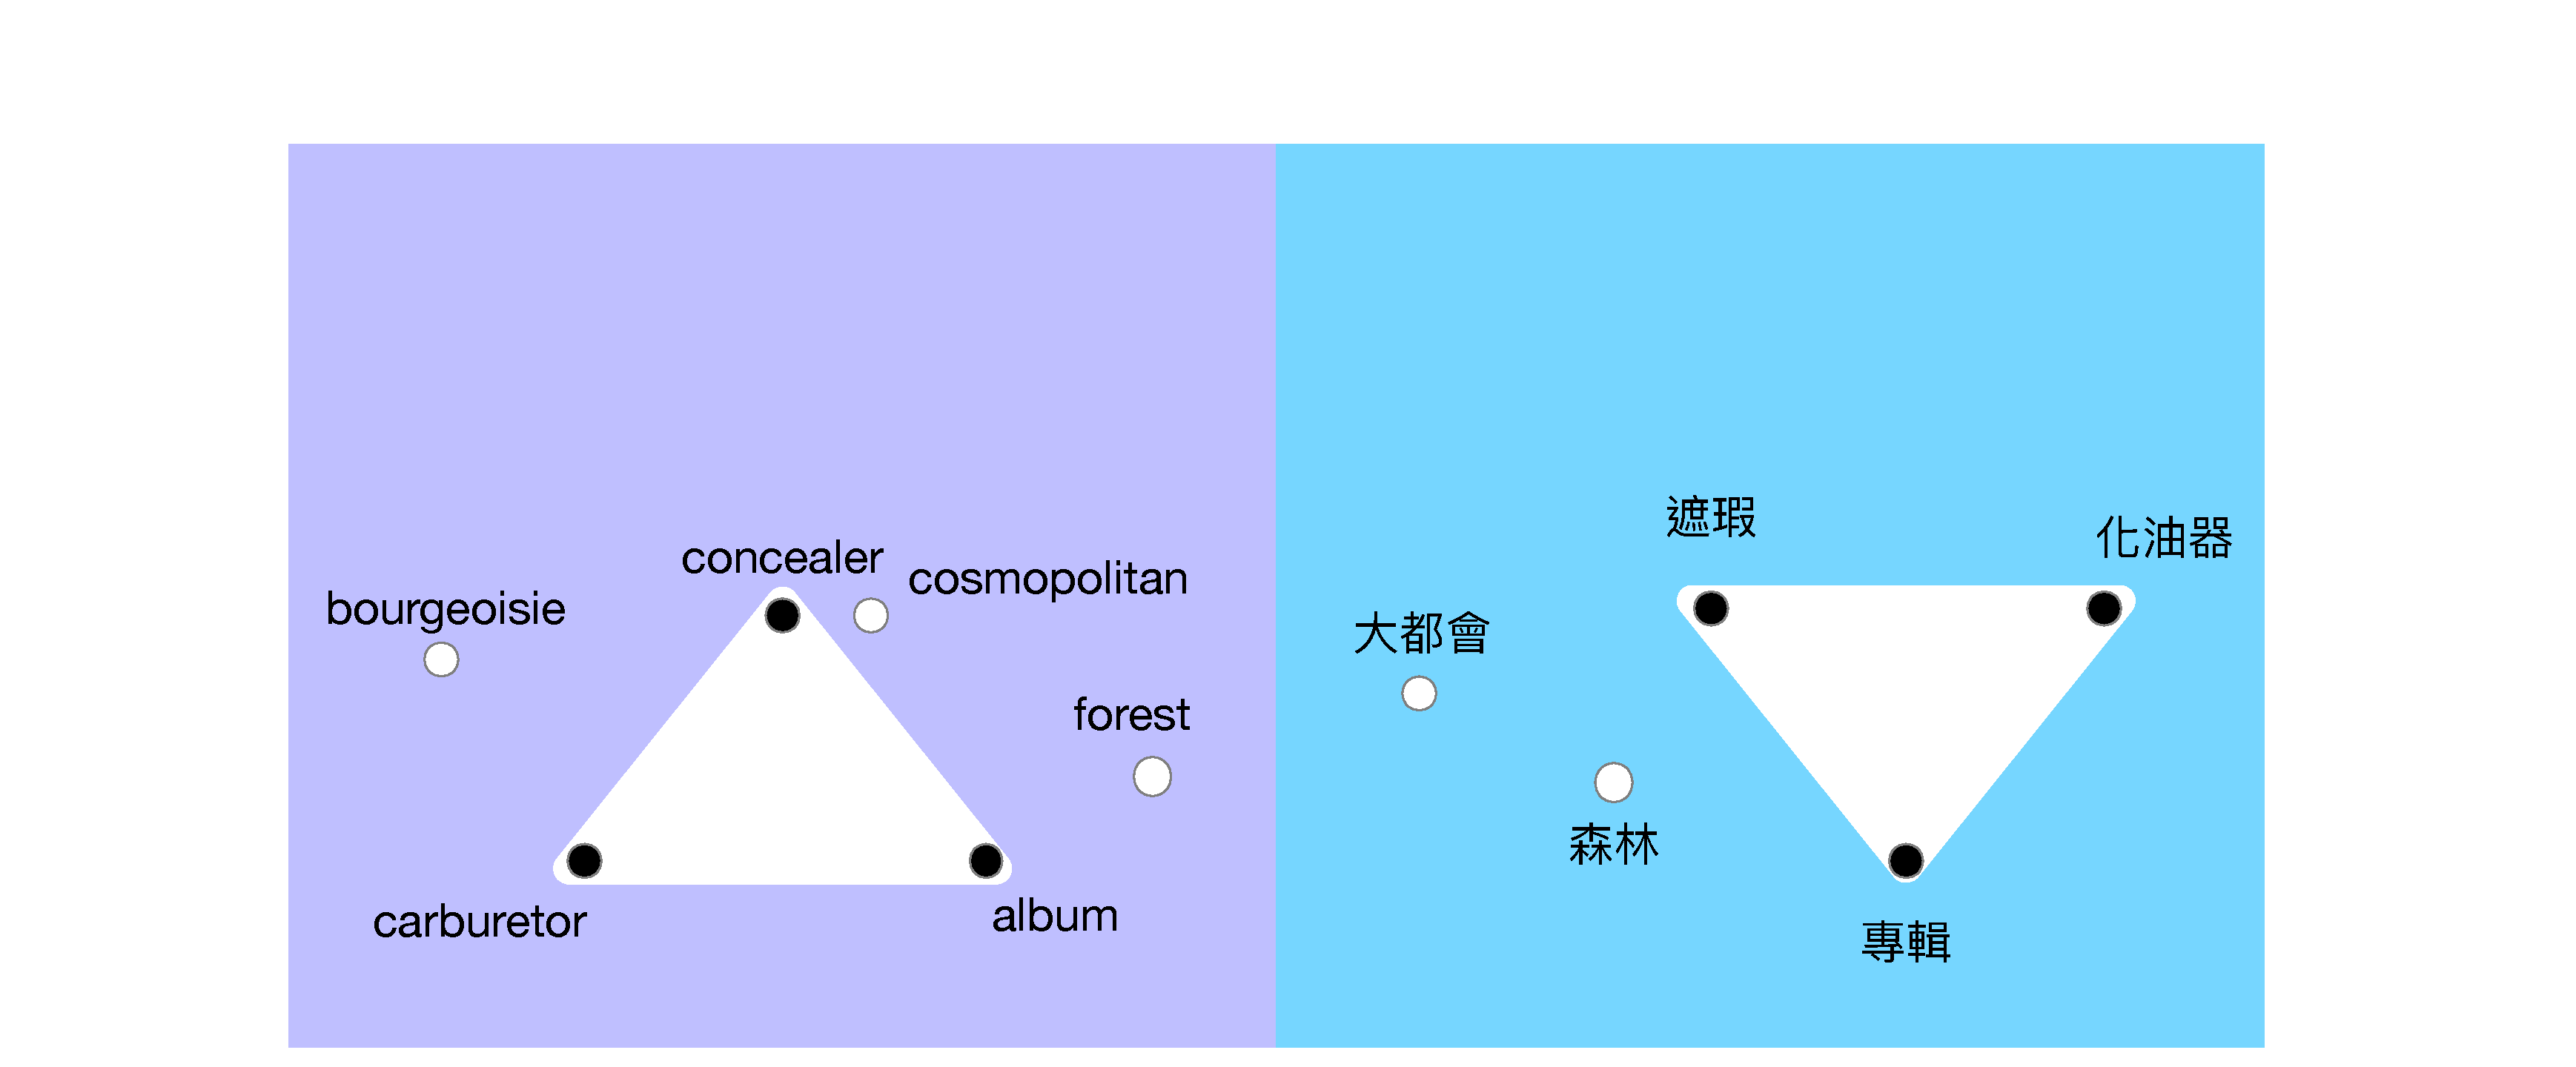
\includegraphics[width=1.2\textwidth]{multi_anchors1.pdf}}
\onslide<2> \centerline{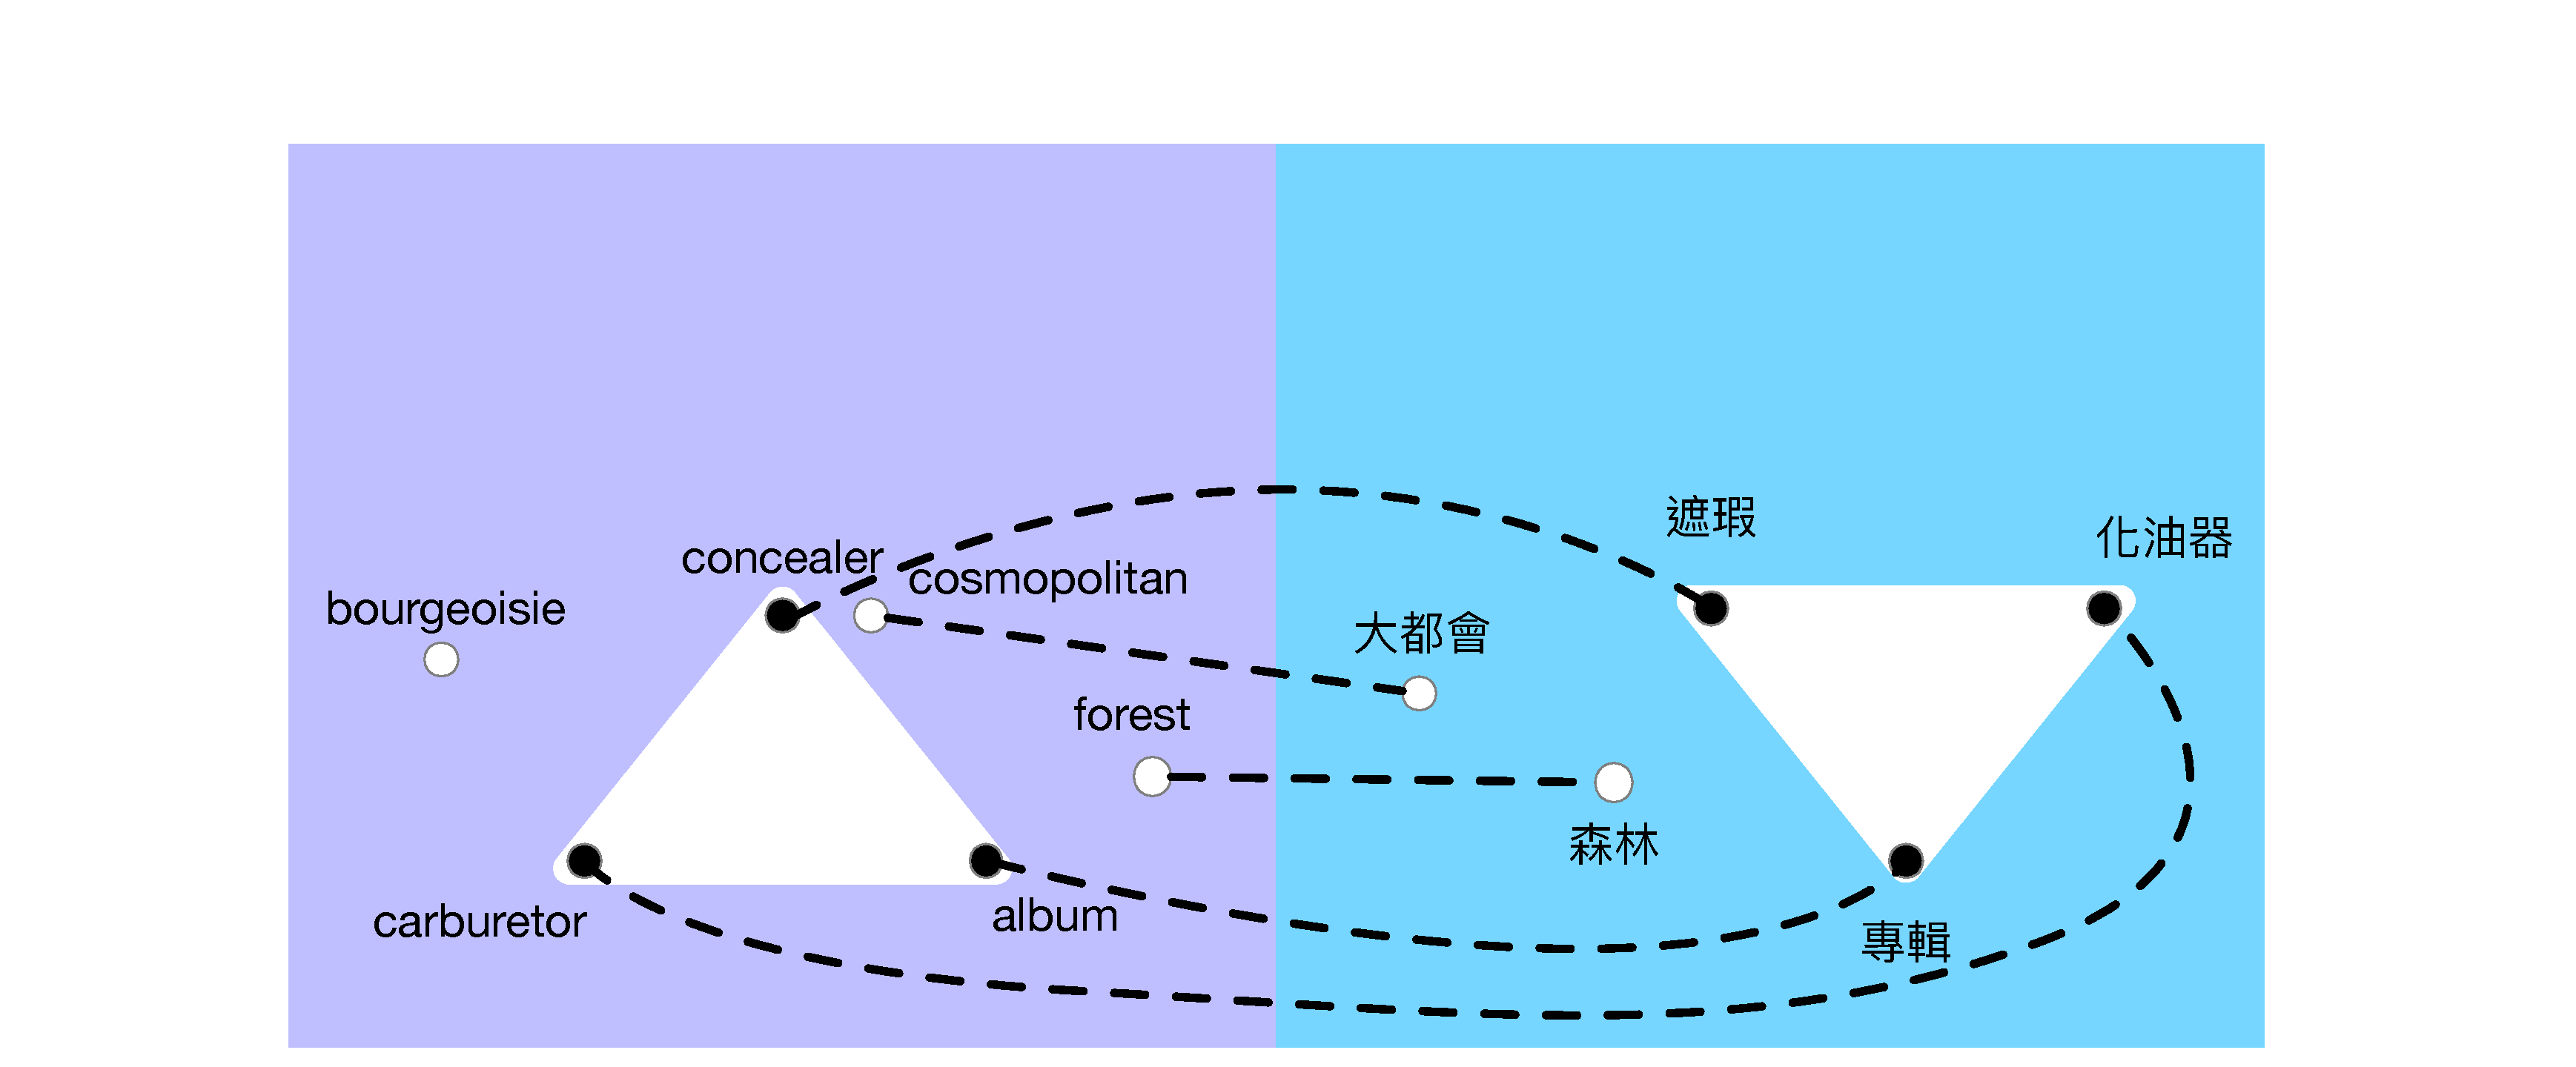
\includegraphics[width=1.2\textwidth]{multi_anchors2.pdf}}
\onslide<3> \centerline{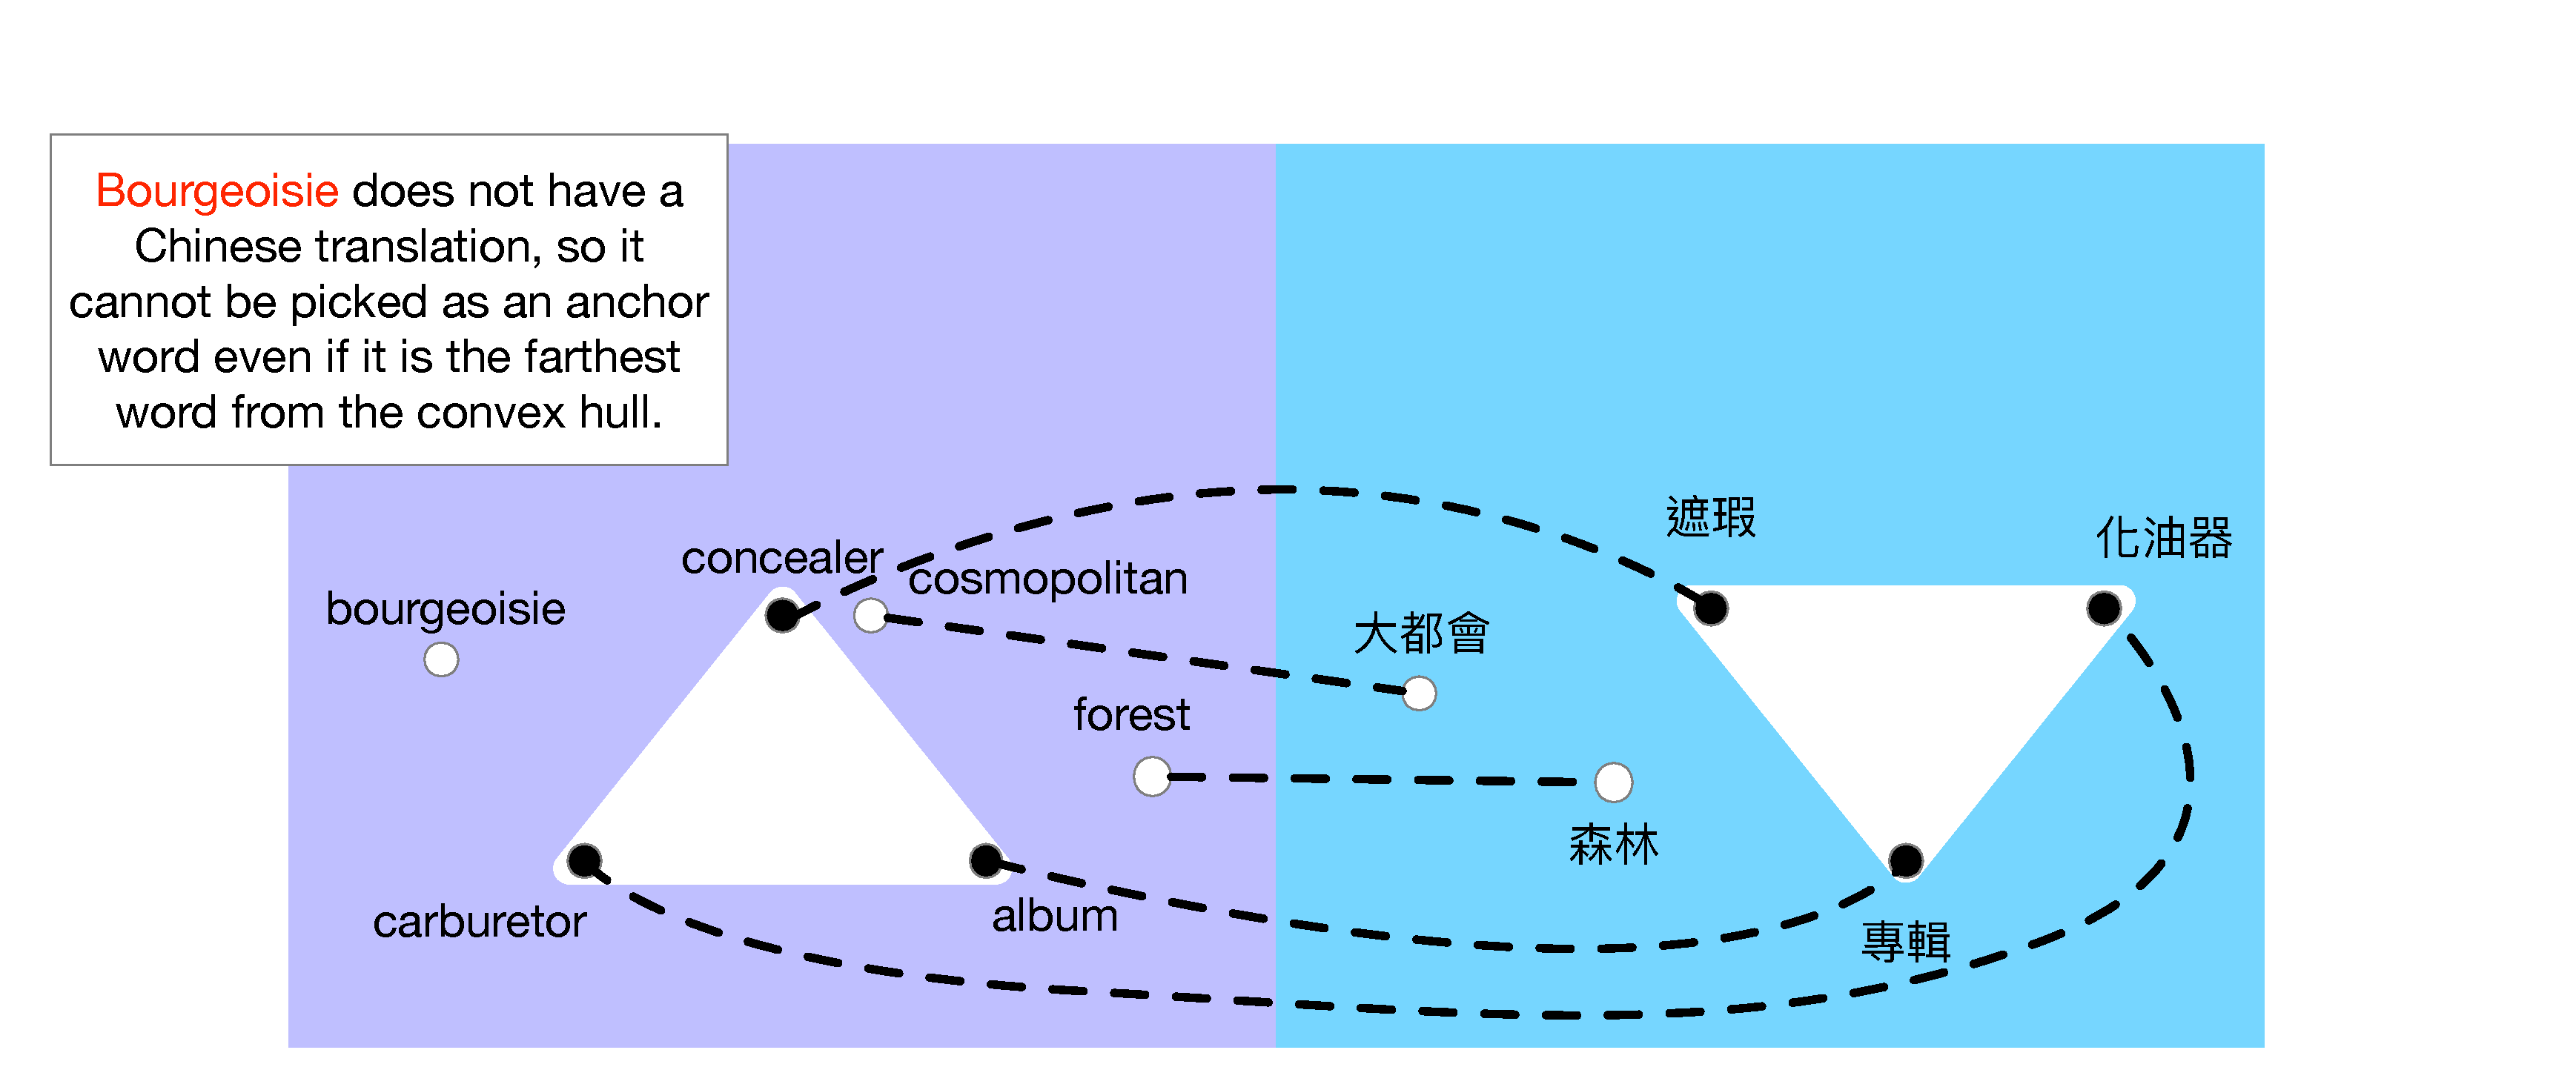
\includegraphics[width=1.2\textwidth]{multi_anchors3.pdf}}
\onslide<4> \centerline{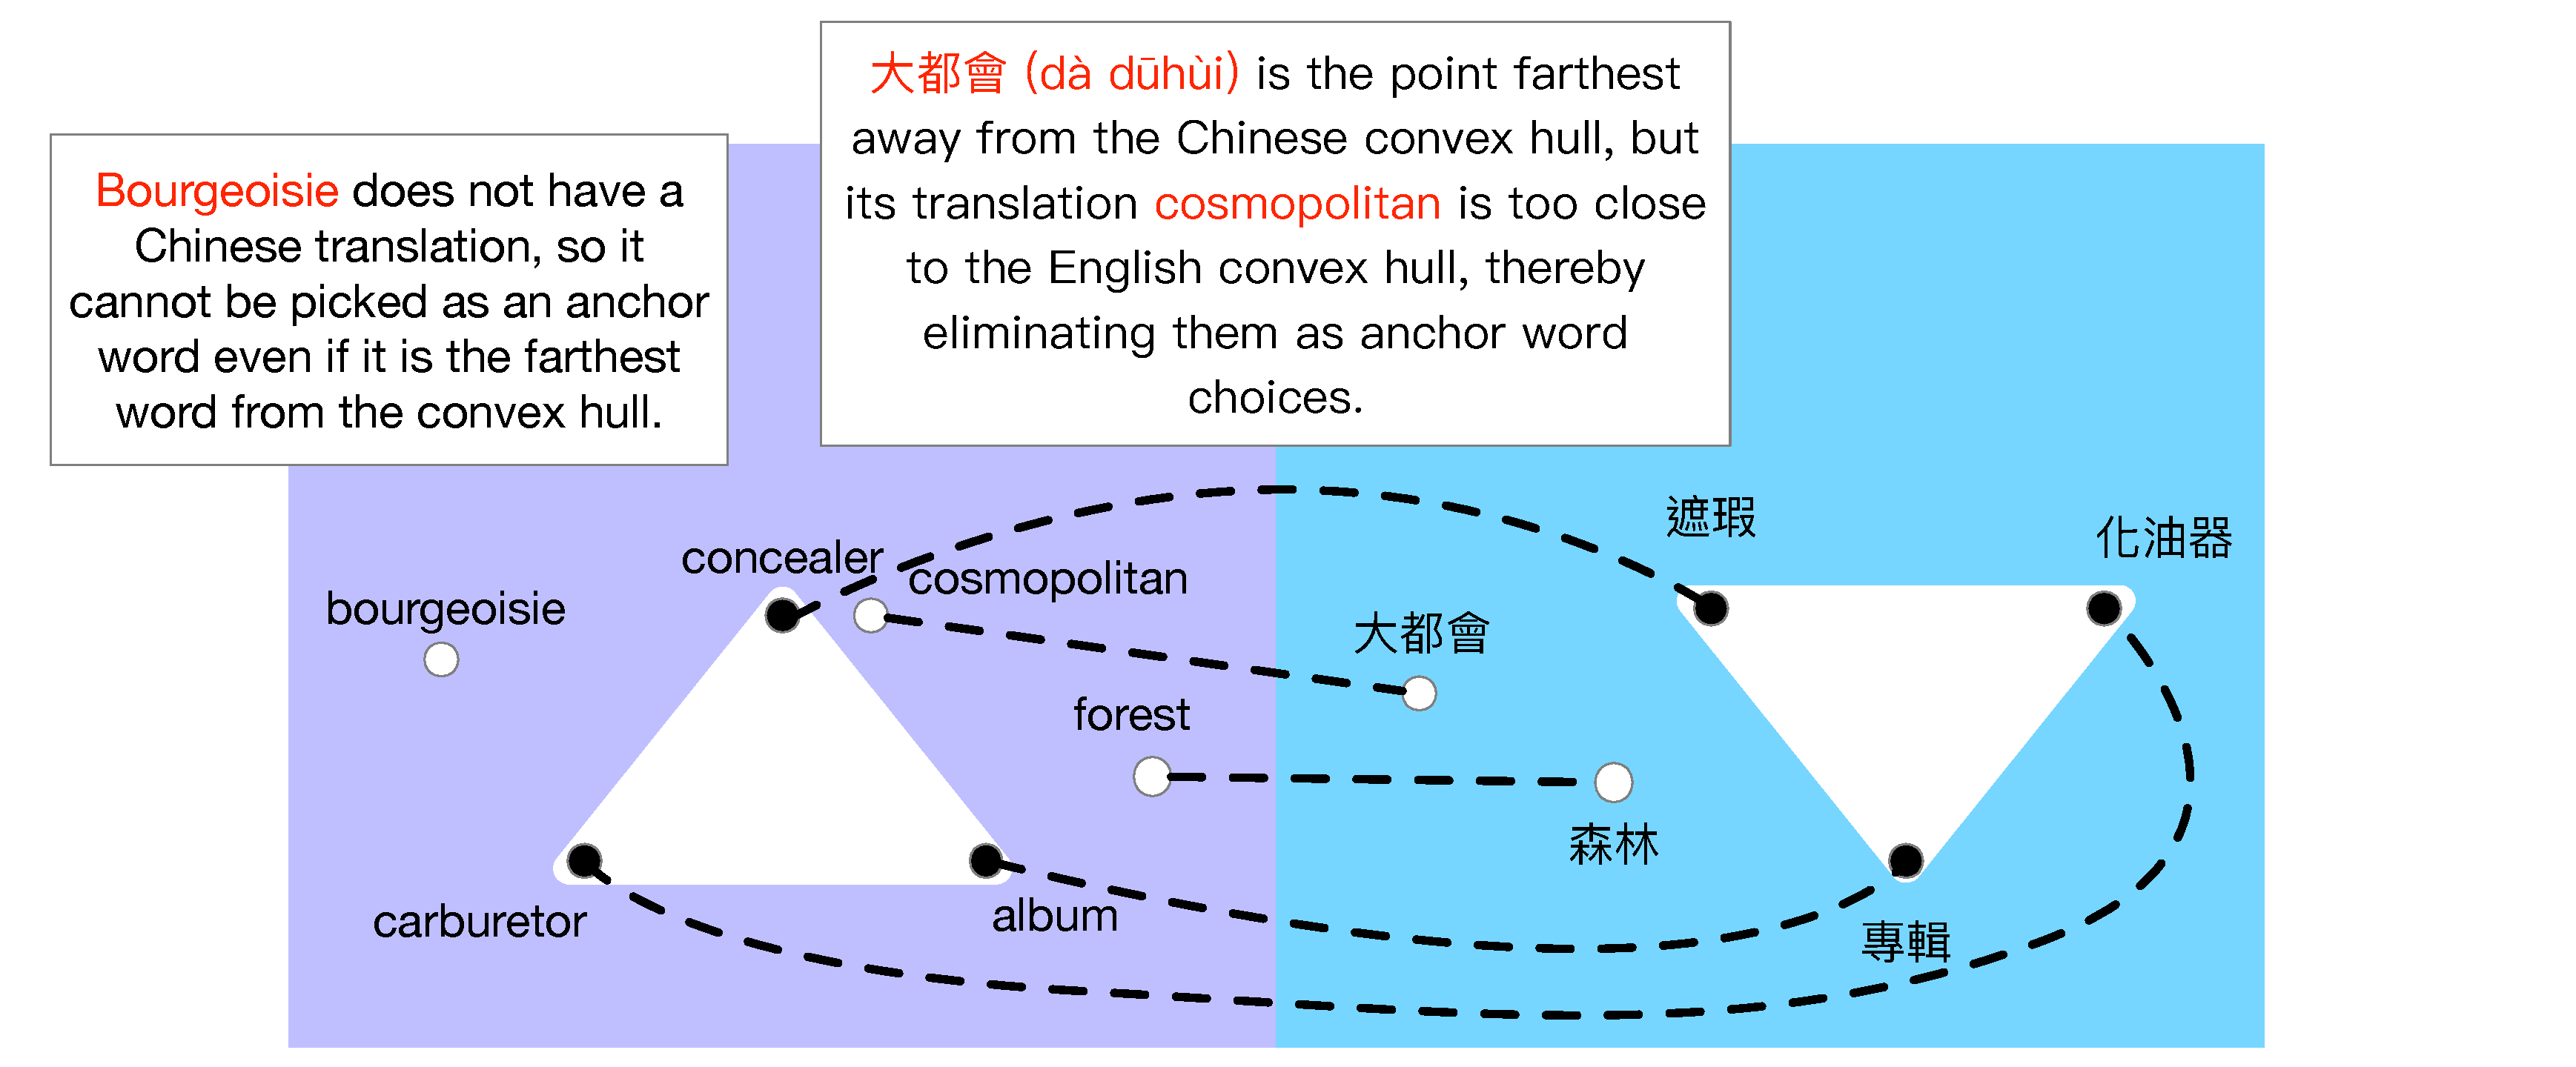
\includegraphics[width=1.2\textwidth]{multi_anchors4.pdf}}
\onslide<5> \centerline{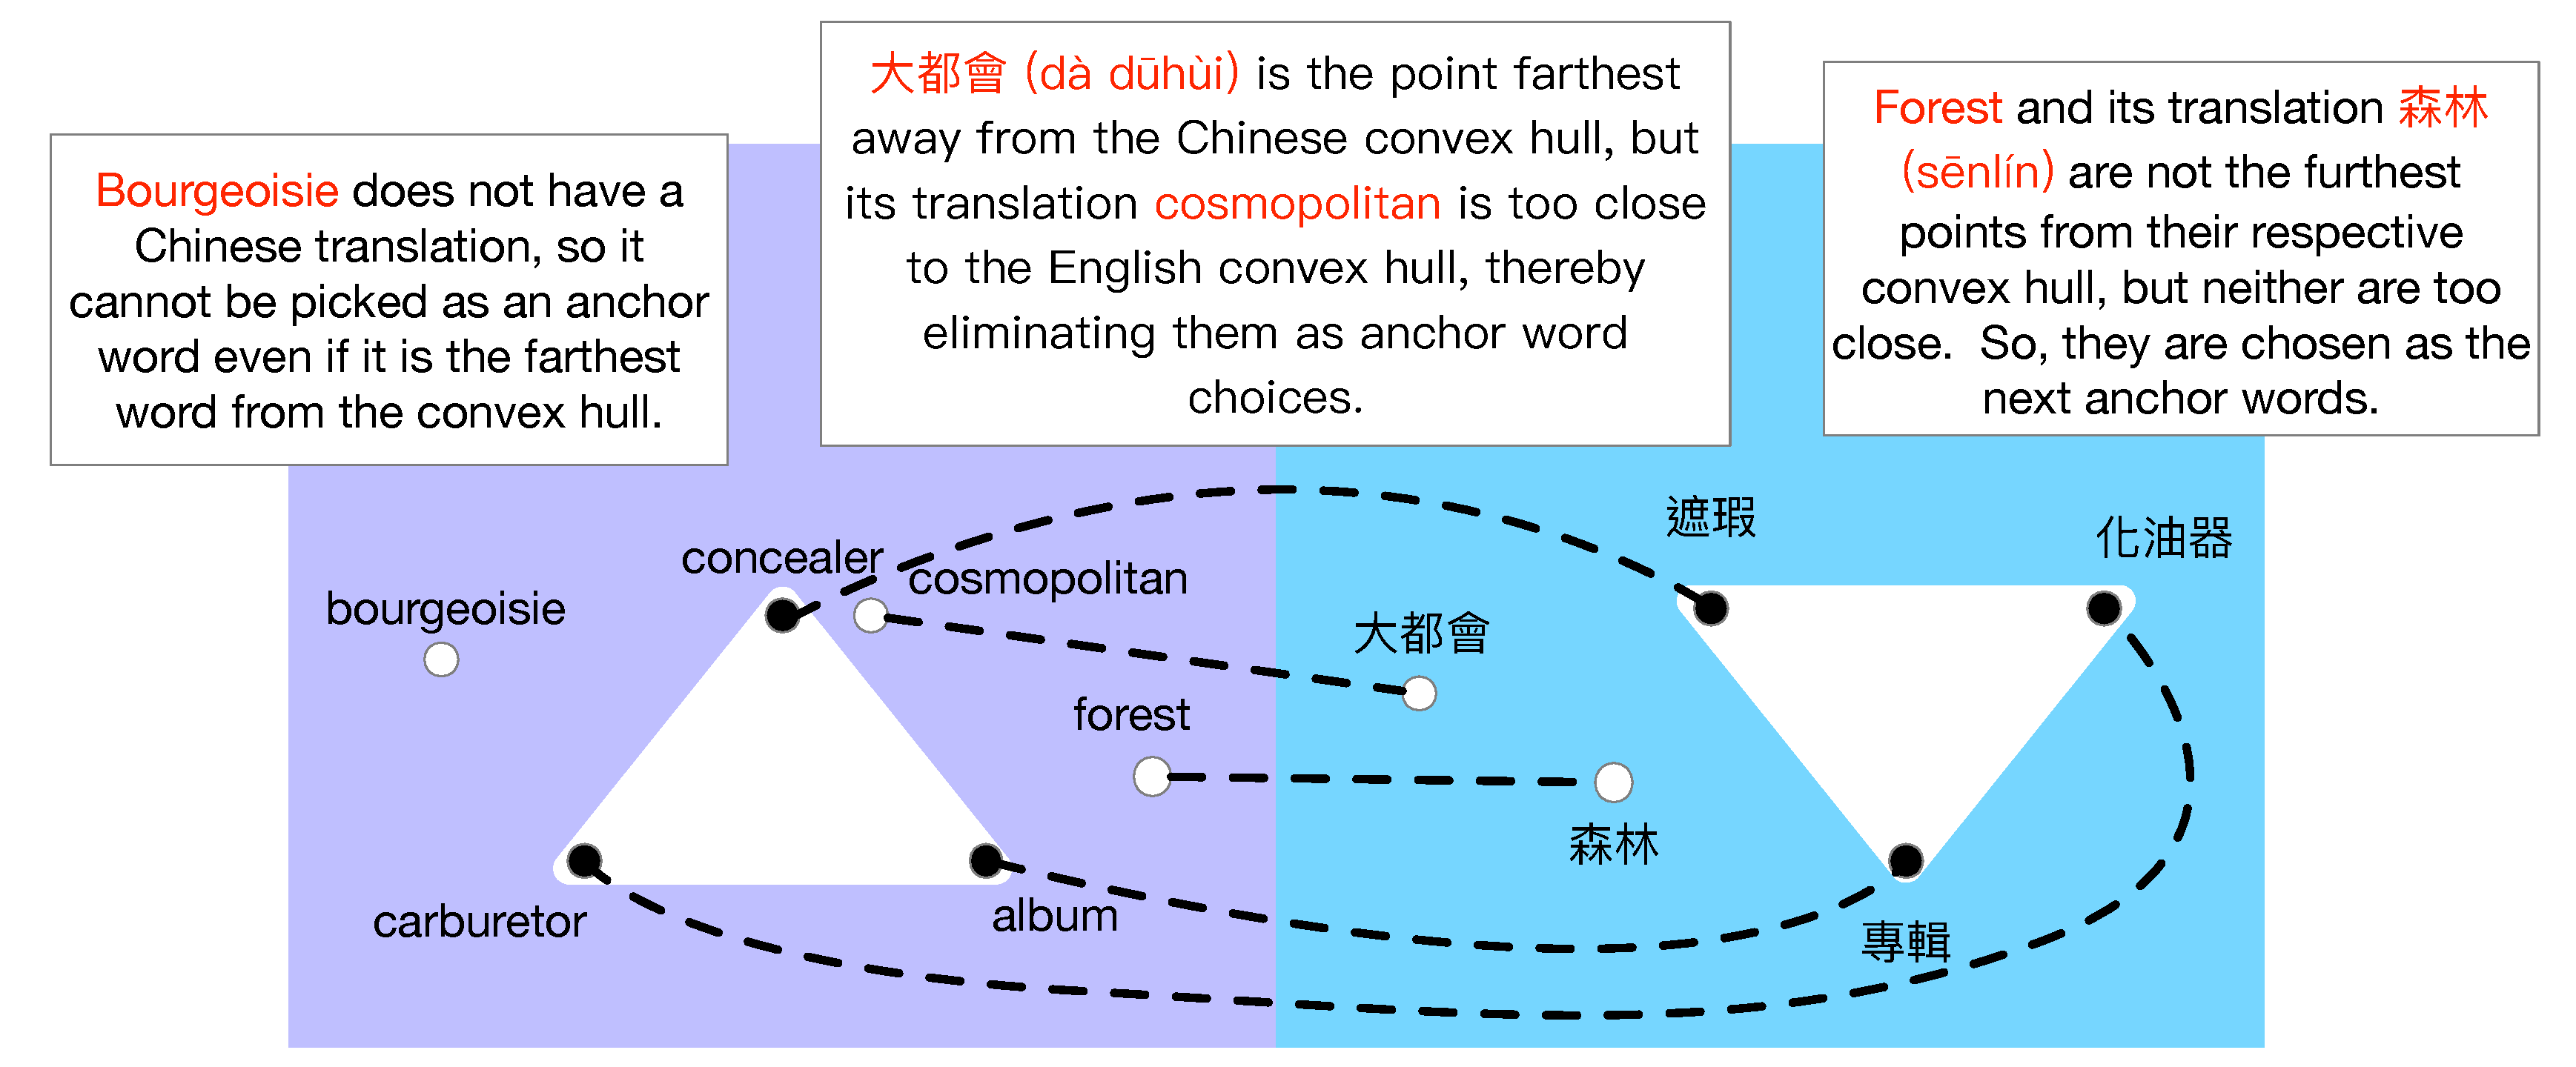
\includegraphics[width=1.2\textwidth]{multi_anchors5.pdf}}
\onslide<6-> \centerline{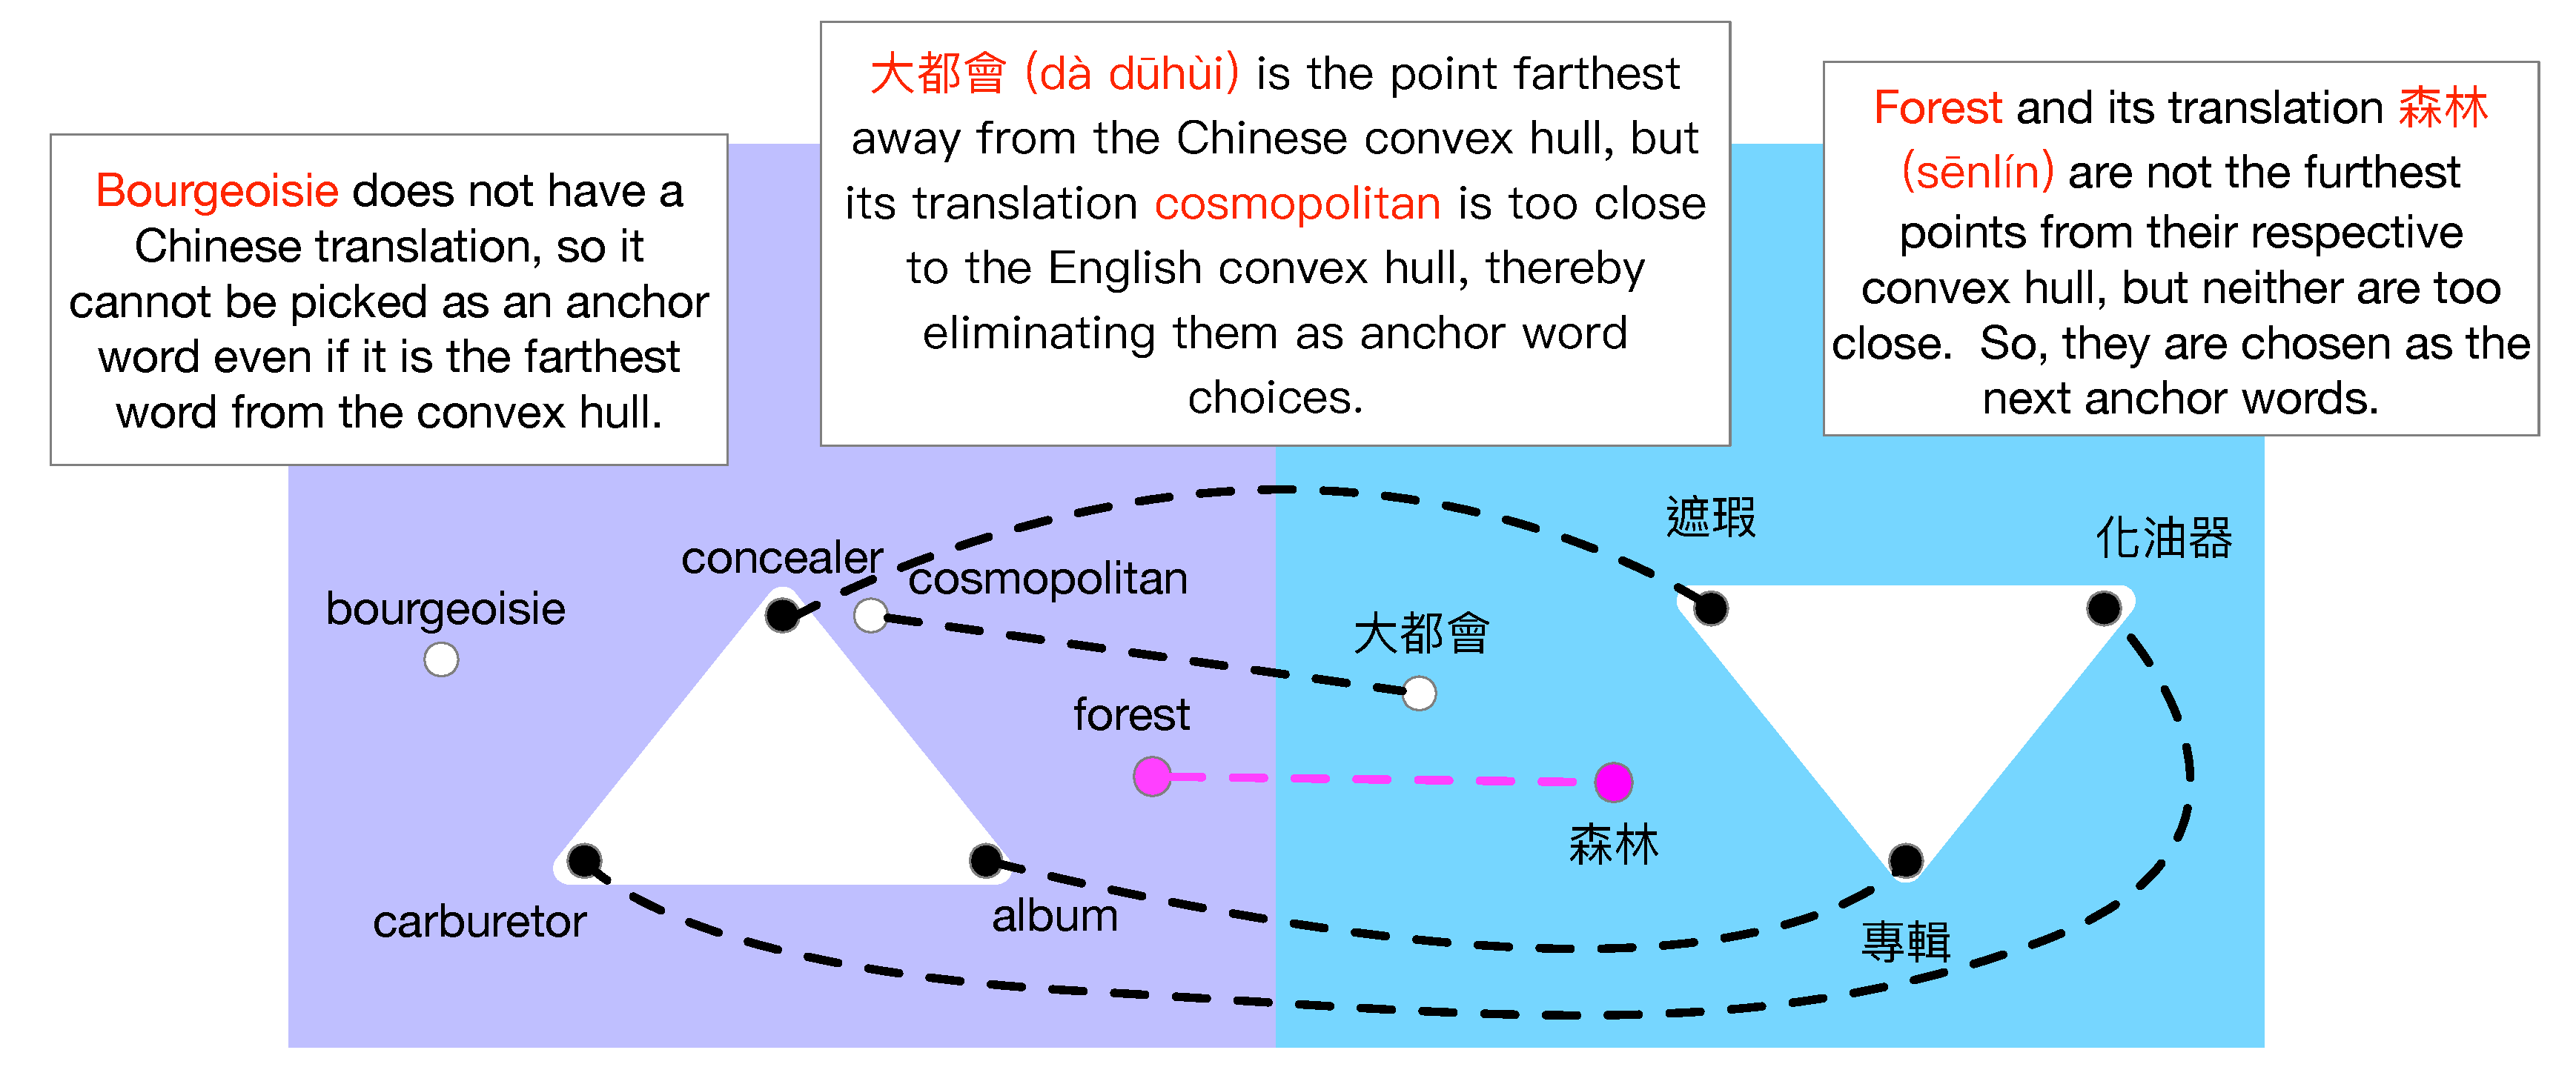
\includegraphics[width=1.2\textwidth]{multi_anchors6.pdf}}
\end{overprint}
\end{figure}
\end{frame}

\begin{frame}{Multilingual Anchoring}
\begin{enumerate}
\item Given a dictionary, create links between words that are translations of each other.
\item Select an anchor word for each language such that the words are linked and span of anchor words is maximized.
\item Once anchor words are found, separately find topic-word distributions for each language.
\end{enumerate}
\end{frame}

\begin{frame}
\begin{itemize}
\item What if dictionary entries are scarce or inaccurate? 
\item What if topics aren't aligned properly across languages?
\end{itemize}
\pause 
\vspace{1cm}
\textbf{Incorporate human-in-the-loop topic modeling tools.}
\end{frame}

\begin{frame}{MTAnchor}
\begin{figure}
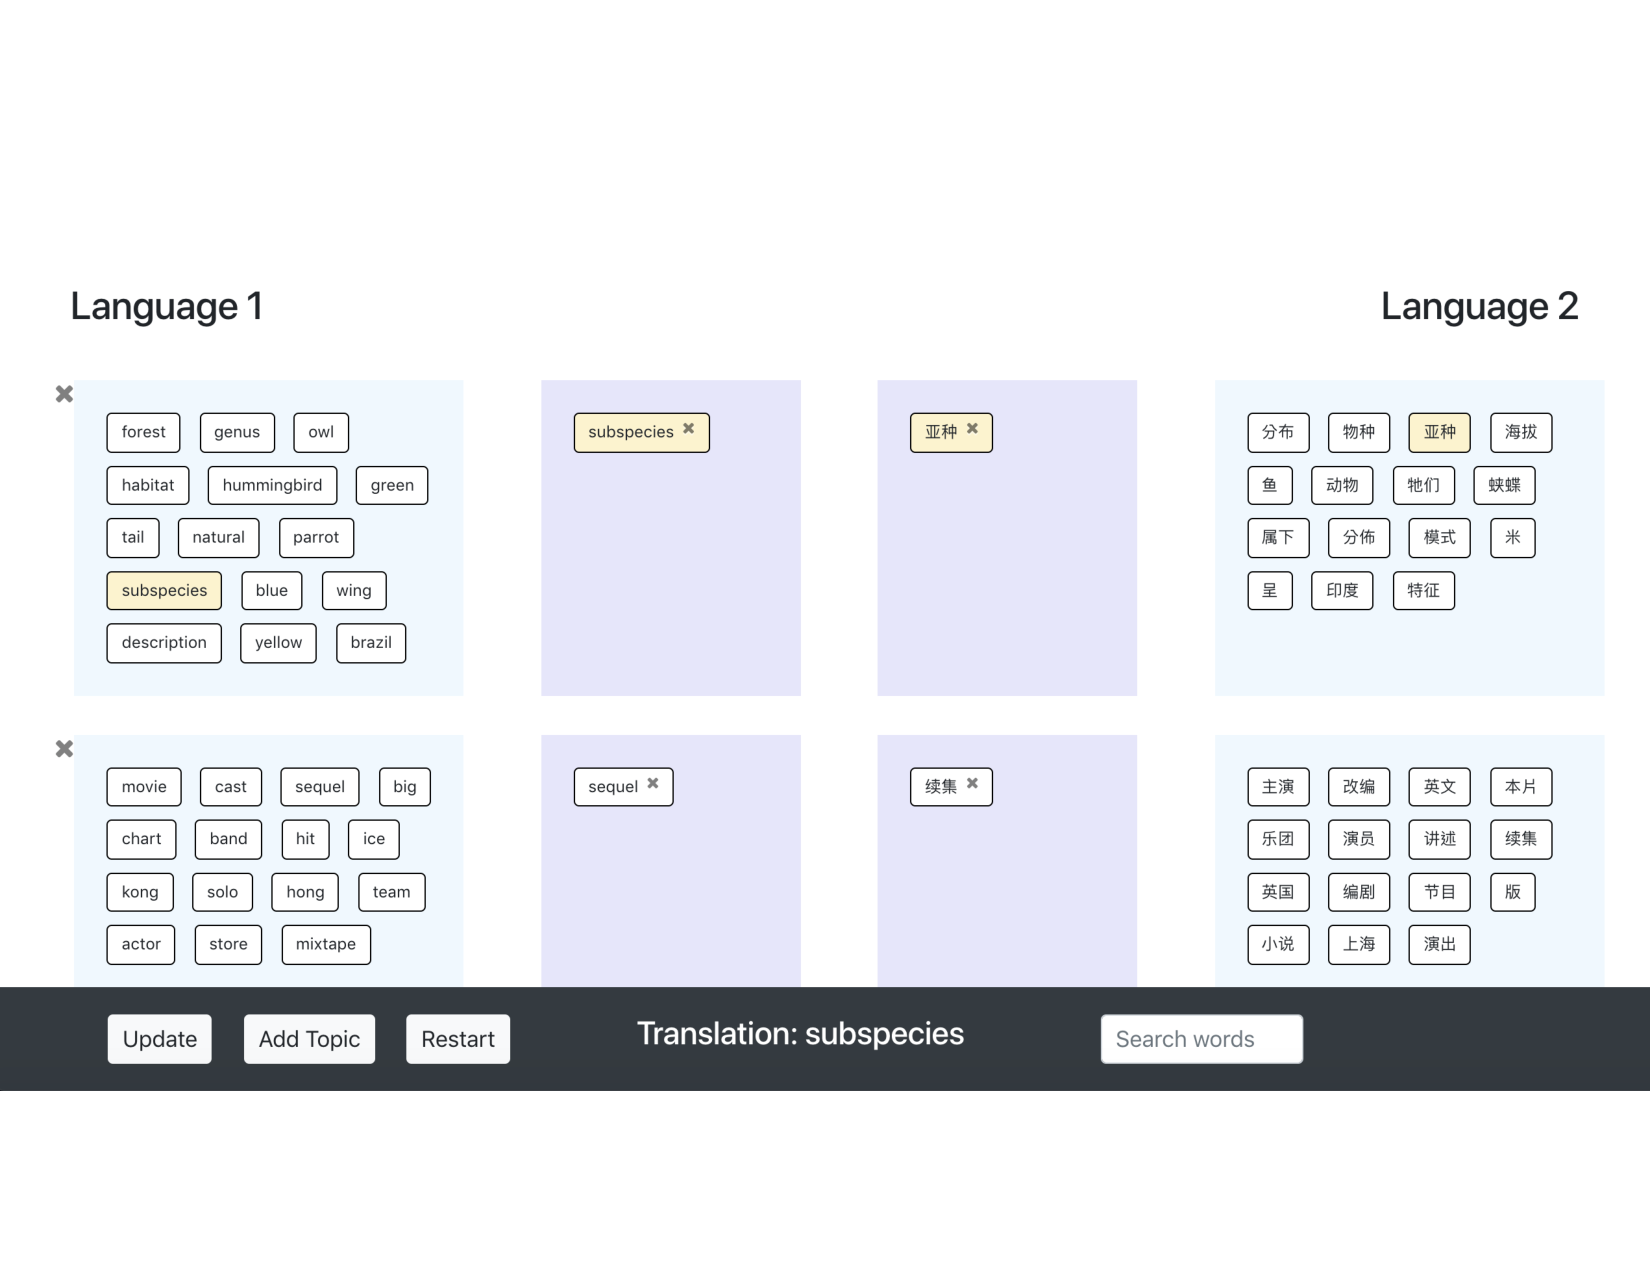
\includegraphics[width=\textwidth]{ui_final.pdf}
\end{figure}
\end{frame}


